\chapter{SocialFramework}
\label{chapter:SocialFramework}

O SocialFramework é uma \textit{engine} do Rails\footnote{\url{http://rubyonrails.org/}} que ajuda a construir redes sociais com recursos comuns e específicos.

O SocialFramework é dividido em três módulos, que são: usuários, rotas e agendas. No módulo de usuários são providos os principais recursos para usuários, como autenticação, registro e pesquisas. No módulo de rotas, o \textit{framework} provê recursos para checar a compatibilidade de rotas. No módulo de agenda, são oferecidos recursos para definir agendas de usuários e a compatibilidade de horários entre usuários.

Portanto, o SocialFramework pode ajudar a construir redes sociais genéricas e específicas, procurando evitar ao usuário, a preocupação com problemas recorrentes nestes tipos de sistemas.

Todo o código desenvolvido do SocialFramework pode ser encontrado no endereço: \url{https://github.com/TCC-SocialNetwork/social_framework}.

A seguir é apresentada uma documentação de todo o funcionamento do SocialFramework, passando pela instalação, uso e interface pública do mesmo.

\section{Instalação}

A instalação do SocialFramework possui dois passos simples.

Primeiro, deve-se adicionar a seguinte linha no arquivo Gemfile:

\begin{lstlisting}[
    label=listing:Gemfile,
    caption=Gemfile,
    numbers=none,
    language=Ruby,
    basicstyle=\footnotesize\sffamily,
    keywordstyle=\color{red},
    stringstyle=\color{blue},
]
gem 'social_framework'
\end{lstlisting}

Após a adição da \textit{gem} no Gemfile, deve-se proceder com a instalação, executando o seguinte comando:

\begin{lstlisting}[
    label=listing:Install,
    caption=Instalação,
    numbers=none,
    language=Bash,
    basicstyle=\footnotesize\sffamily,
    keywordstyle=\color{red},
    stringstyle=\color{blue},
]
$ bundle install
\end{lstlisting}

Tal procedimento irá instalar o SocialFramework na aplicação.

Nas seções a seguir, será apresentado o funcionamento do SocialFramework como um \textit{framework} do tipo caixa preta e do tipo caixa cinza. Mais especificamente, nas seções ~\nameref{sec:primeiros_passos} e \nameref{sec:modulos_socialframework}, será apresentado seu uso como um \textit{framework} caixa preta. Já na seção \nameref{sec:hotspots}, será apresentado o seu uso como um \textit{framework} caixa cinza.

\section{Primeiros Passos}
\label{sec:primeiros_passos}

O uso do SocialFramework é indicado para quem já possui algum conhecimento do \textit{framework} Rails para um maior entendimento e aproveitamento de seus recursos fornecidos.

O SocialFramework utiliza o Devise\footnote{\url{https://github.com/plataformatec/devise}}, que é uma solução de autenticação flexível para Rails. Toda a documentação do Devise pode ser encontrada no repositório do projeto no GitHub, no endereço \url{https://github.com/plataformatec/devise}.

A classe de usuário foi implementada no SocialFramework, e possui algumas diferenças da classe de usuário padrão do Devise, como a adição do atributo nome e dos relacionamentos dos usuários. As \textit{controllers} e \textit{views} do Devise também foram alteradas para adicionar os novos recursos.

Inicialmente, alguns arquivos devem ser adicionados na aplicação para que as configurações do SocialFramework e do Devise sejam importadas. Esses arquivos são os \textit{initializers}, o arquivo de internacionalização (i18n) do Devise, as rotas e as \textit{views} de \textit{registration} e \textit{session} para criar e autenticar usuários. Para isso deve-se executar:

\begin{lstlisting}[
    label=listing:generate_social_framework,
    caption=Gerando as configurações do SocialFramework e do Devise,
    numbers=none,
    language=Bash,
    basicstyle=\footnotesize\sffamily,
    keywordstyle=\color{red},
    stringstyle=\color{blue},
]
$ rails generate social_framework:install
\end{lstlisting}

Este comando irá criar o arquivo ``config/initializers/devise.rb'', contendo as configurações do Devise; o arquivo ``config/initializers/social\_framework.rb'', que contém as configurações do SocialFramework; o arquivo i18n do Devise, e irá adicionar a rota ``devise\_for'', para mapear as \textit{controllers} e \textit{views} do Devise. Dessa forma, a aplicação estará preparada para usar o módulo de usuários com as configurações e comportamentos padrões.

Todas as tabelas do \textit{framework} deverão criadas no banco de dados da aplicação. Portanto, para testar a aplicação não se deve esquecer de executar as \textit{migrations}:

\begin{lstlisting}[
    label=listing:migrations,
    caption=Migrations,
    numbers=none,
    language=Bash,
    basicstyle=\footnotesize\sffamily,
    keywordstyle=\color{red},
    stringstyle=\color{blue},
]
$ rake db:create
$ rake db:migrate
\end{lstlisting}

Para acessar a página de autenticação, deve-se acessar a rota ``/users/sign\_in''. Esta página está preparada para autenticar usuários com \textit{email} ou nome de usuário. Para cadastrar um novo usuário, deve-se acessar a rota ``/users/sign\_up''. Ao criar um novo usuário, este estará automaticamente conectado.

Quando se usa o Devise Mailer como o módulo de confirmação, é necessário adicionar em seu ambiente as configurações para a ação \textit{mailer}. Por exemplo, se estiver no ambiente de desenvolvimento, deve-se adicionar as seguintes configurações no arquivo `development.rb'.

\begin{lstlisting}[
    label=listing:mailer,
    caption=Configurações de email,
    numbers=left,
    language=Ruby,
    basicstyle=\footnotesize\sffamily,
    keywordstyle=\color{red},
    stringstyle=\color{blue},
    showspaces=false,
    showstringspaces=false,
]
config.action_mailer.default_url_options = {host: 'localhost', port: 3000}

config.action_mailer.delivery_method = :smtp

config.action_mailer.smtp_settings = {
  address: "smtp.gmail.com",
  port: 587,
  domain: ENV["GMAIL_DOMAIN"],
  authentication: "plain",
  enable_starttls_auto: true,
  user_name: ENV["GMAIL_USERNAME"],
  password: ENV["GMAIL_PASSWORD"]
}
\end{lstlisting}

Pode-se alterar os valores em `domain', `user\_name', e `password' ou criar as variáveis de ambiente locais, sendo indicado para esconder essas informações sigilosas e garantir uma maior segurança. As mesmas configurações são válidas para os ambientes de teste e produção, nos arquivos `test.rb' e `production.rb'.

\subsection{Controller Filters and Helpers}

O Devise fornece alguns elementos para serem usados nas \textit{controllers} e \textit{views}. Para configurar uma \textit{controller} com uma autenticação de usuário, basta adicionar o seguinte filtro. Isto funciona porque o SocialFramework já contém a classe de usuário.

\begin{lstlisting}[
    label=listing:authenticate,
    caption=Requer autenticação de usuário,
    numbers=none,
    language=Ruby,
    basicstyle=\footnotesize\sffamily,
    keywordstyle=\color{red},
    stringstyle=\color{blue},
    showspaces=false,
    showstringspaces=false,
]
before_action :authenticate_user!
\end{lstlisting}

Outros elementos são:

\begin{lstlisting}[
    label=listing:signed_in,
    caption=Verifica se o usuário está logado,
    numbers=none,
    language=Ruby,
    basicstyle=\footnotesize\sffamily,
    keywordstyle=\color{red},
    stringstyle=\color{blue},
    showspaces=false,
    showstringspaces=false,
]
user_signed_in?
\end{lstlisting}

\begin{lstlisting}[
    label=listing:current_user,
    caption=Recupera o usuário logado,
    numbers=none,
    language=Ruby,
    basicstyle=\footnotesize\sffamily,
    keywordstyle=\color{red},
    stringstyle=\color{blue},
    showspaces=false,
    showstringspaces=false,
]
current_user
\end{lstlisting}

\begin{lstlisting}[
    label=listing:user_session,
    caption=Recupera a sessão para este escopo,
    numbers=none,
    language=Ruby,
    basicstyle=\footnotesize\sffamily,
    keywordstyle=\color{red},
    stringstyle=\color{blue},
    showspaces=false,
    showstringspaces=false,
]
user_session
\end{lstlisting}

Após o usuário logar, confirmar a conta ou atualizar a senha, o Devise irá procurar por um caminho \textit{root} para redirecionar. Para alterar esse comportamento padrão, pode-se sobrescrever os métodos ``after\_sing\_in\_path\_for'' e ``after\_sing\_out\_path\_for'', para definir para onde o usuário deve ser redirecionado após realizar o \textit{login} e o \textit{logout} respectivamente.

\subsection{Configuração das Modelos}
\label{configuracao_das_modelos}

A classe de usuário no SocialFramework implementa os módulos padrões do Devise. Na documentação completa do Devise, é possível encontrar todos os módulos e suas características.

Além dos módulos do Devise, a classe de usuário do SocialFramework possui métodos que implementam os comportamentos para os relacionamentos de usuários. É possível sobrescrever qualquer comportamento, estendendo a classe em outra modelo, como:

\begin{lstlisting}[
    label=listing:extensao_user_class,
    caption=Estensão da classe de usuário,
    numbers=none,
    language=Ruby,
    basicstyle=\footnotesize\sffamily,
    keywordstyle=\color{red},
    stringstyle=\color{blue},
    showspaces=false,
    showstringspaces=false,
]
class OtherUserClass < SocialFramework::User
  # Your code goes here
end
\end{lstlisting}

É necessário mudar o nome da classe no arquivo ``routes.rb'' para a nova classe criada, assim o Devise poderá enxergar a nova classe. Para fazer isso:

\begin{lstlisting}[
    label=listing:devise_new_user_class,
    caption=Configurando a nova classe de usuário para o Devise,
    numbers=none,
    language=Ruby,
    basicstyle=\footnotesize\sffamily,
    keywordstyle=\color{red},
    stringstyle=\color{blue},
    showspaces=false,
    showstringspaces=false,
]
devise_for :users, class_name: 'OtherUserClass',
    controllers: {sessions: 'users/sessions',
                  registrations: 'users/registrations',
                  passwords: 'users/passwords'}
\end{lstlisting}

Além disso, deve-se colocar o nome da nova classe de usuário também no arquivo ``social\_framework.rb'' para que o \textit{factory} das classes de modelo possa funcionar adequadamente. Nesse caso, deve-se alterar a linha com o nome da classe de usuário deixando-a:

\begin{lstlisting}[
    label=listing:change_user_class_name,
    caption=Configurando a nova classe de usuário para o \textit{framework},
    numbers=none,
    language=Ruby,
    basicstyle=\footnotesize\sffamily,
    keywordstyle=\color{red},
    stringstyle=\color{blue},
    showspaces=false,
    showstringspaces=false,
]
config.user_class = 'OtherUserClass'
\end{lstlisting}

Maiores detalhes sobre esse aspecto podem ser encontrados na seção \nameref{sec:hotspots}.

\subsection{Configuração das Migrations}
\label{configuracao_das_migrations}

A classe de usuário fornece como padrão os atributos nome de usuário, \textit{e-mail} e senha. Para adicionar ou remover atributos para esta ou qualquer outra classe, pode-se adicionar a \textit{migrate} na aplicação. O SocialFramework dispõe de um gerador, sendo, neste caso, necessário executar:

\begin{lstlisting}[
    label=listing:generate_migrate,
    caption=Geração das \textit{migrations},
    numbers=none,
    language=Bash,
    basicstyle=\footnotesize\sffamily,
    keywordstyle=\color{red},
    stringstyle=\color{blue},
    showspaces=false,
    showstringspaces=false,
]
$ rails generate social_framework:install_migrations -m users
\end{lstlisting}

A \textit{migrate} de usuário será adicionada na aplicação e poderá ser alterada. O parâmetro `-m' é usado para gerar \textit{migrations} específicas. O \textit{script} espera os nomes das \textit{migrations}. Caso não exista a \textit{migration} na aplicação, esta será gerada.

Caso seja adicionado ou removido um atributo para o usuário, deve-se notificar o Devise, usando um filtro \textit{before} na ``ApplicationController'':

\begin{lstlisting}[
    label=listing:user_attribute,
    caption=Configuração para adicionar um novo atributo de usuário,
    numbers=none,
    language=Ruby,
    basicstyle=\footnotesize\sffamily,
    keywordstyle=\color{red},
    stringstyle=\color{blue},
    showspaces=false,
    showstringspaces=false,
]
class ApplicationController < ActionController::Base
  before_action :configure_permitted_parameters, if: :devise_controller?

  protected

  def configure_permitted_parameters
    devise_parameter_sanitizer.for(:sign_up) << :new_attribute
    devise_parameter_sanitizer.for(:account_update) << :new_attribute
  end
end
\end{lstlisting}

Isto faz com que o \textit{sign\_up} e o \textit{account\_update} receba o novo atributo. Pode-se usar o método de remoção para remover os atributos existentes. Para adicionar ou remover o parâmetro em outras ações, por exemplo o \textit{sign\_in}, deve-se fazer o mesmo procedimento.

\subsection{Configuração das Controllers}

Todas as \textit{controllers} do Devise podem ser estendidas e ter o seus métodos sobrescritos. Por exemplo:

\begin{lstlisting}[
    label=listing:extensao_controller,
    caption=Estensão de uma controller,
    numbers=none,
    language=Ruby,
    basicstyle=\footnotesize\sffamily,
    keywordstyle=\color{red},
    stringstyle=\color{blue},
    showspaces=false,
    showstringspaces=false,
]
class OtherRegistrationControllerClass < Users::RegistrationsController
  # Your code goes here
end
\end{lstlisting}

Outras \textit{controllers} são: ``confirmations'', ``omniauth\_callbacks'', ``passwords'', ``sessions'' e ``unlocks''. Para usar os módulos de ``omniauth\_callbacks'', ``unlocks'' e ``confirmations'', é necessário adicionar esses respectivos módulos do Devise na aplicação. Todas as \textit{controllers} do Devise no SocialFramework possuem o prefixo ``Users''.

\subsection{Configuração das Rotas}

Quando se substitui algumas \textit{controllers} do Devise deve-se definir essas novas \textit{controllers} nas rotas. Isto pode ser feito alterando o caminho para a \textit{controller} na configuração \textit{devise\_for}, como no exemplo a seguir:

\begin{lstlisting}[
    label=listing:configuracao_controller,
    caption=Configuração de uma \textit{controller},
    numbers=none,
    language=Ruby,
    basicstyle=\footnotesize\sffamily,
    keywordstyle=\color{red},
    stringstyle=\color{blue},
    showspaces=false,
    showstringspaces=false,
]
devise_for :users, class_name: 'SocialFramework::User',
  controllers: {sessions: 'users/sessions',
                registrations: 'new_registration_controller_path',
                passwords: 'users/passwords'}
\end{lstlisting}

A \textit{controller} de registro foi estendida, e a nova \textit{controller} foi adicionada nas configurações de rotas do Devise.

\subsection{Configuração das Views}

Para adicionar as \textit{views} do Devise na aplicação, o SocialFramework possui um gerador para executar esta tarefa. Para executá-lo, deve-se usar o seguinte comando:

\begin{lstlisting}[
    label=listing:gerar_views,
    caption=Geração das \textit{views},
    numbers=none,
    language=Bash,
    basicstyle=\footnotesize\sffamily,
    keywordstyle=\color{red},
    stringstyle=\color{blue},
    showspaces=false,
    showstringspaces=false,
]
$ rails generate social_framework:views
\end{lstlisting}

Para adicionar uma \textit{view} específica, deve-se usar o parâmetro `-v', e passar o nome das \textit{views}, como no exemplo a seguir:

\begin{lstlisting}[
    label=listing:gerar_views,
    caption=Geração das \textit{views},
    numbers=none,
    language=Bash,
    basicstyle=\footnotesize\sffamily,
    keywordstyle=\color{red},
    stringstyle=\color{blue},
    showspaces=false,
    showstringspaces=false,
]
$ rails generate social_framework:views -v registrations sessions passwords
\end{lstlisting}

Este comando irá adicionar as \textit{views} ``registrations'', ``sessions'' e ``passwords'' na aplicação. Outras \textit{views} são: ``confirmations'', ``mailer'' e ``unlocks''. Inicialmente, o SocialFramework adiciona as \textit{views} ``registrations'' e ``sessions'' na aplicação, fornecendo autenticação e registro para os usuários.

\section{Módulos do SocialFramework}
\label{sec:modulos_socialframework}

Atualmente, o SocialFramework possui os módulos de usuário, de rotas e de agendas. Estes módulos serão detalhados a seguir.

\subsection{Módulo de Usuários}

Este módulo fornece a lógica principal às redes sociais, como criar, confirmar e remover relacionamentos entre os usuários, além de buscas, registros, atualizações e autenticações.

A estrutura de relacionamentos foi construída com um relacionamento de muitos para muitos entre usuários, através de arestas. As arestas possuem: o usuário de origem; o usuário de destino; o \textit{status}, o qual pode estar ativo ou inativo; se é bidirecional ou não, o que  especifica se um relacionamento é bidirecional ou unidirecional, e um rótulo com o nome do relacionamento. Podem existir múltiplos relacionamentos entre os mesmos usuários. Cada relacionamento é representado com uma aresta.

Para criar um novo relacionamento entre dois usuários, deve-se utilizar o método `create\_relationship', definido na classe de usuário. Esse método possui a seguinte assinatura:

\begin{lstlisting}[
    label=listing:create_relationship,
    caption=Método para criar relacionamento,
    numbers=none,
    language=Ruby,
    basicstyle=\footnotesize\sffamily,
    keywordstyle=\color{red},
    stringstyle=\color{blue},
    showspaces=false,
    showstringspaces=false,
]
create_relationship(destiny, label, bidirectional=true, active=false)
\end{lstlisting}

O usuário que pede o relacionamento deve chamar este método e passar o usuário de destino e rótulo para o relacionamento. Por padrão, é criado um relacionamento bidirecional e inativo entre esses usuários. É possível mudar esse comportamento passando outros parâmetros para o método.

Para ativar o relacionamento criado, é necessária uma confirmação. Assim, o usuário de destino deve invocar o método `confirm\_relationship'. Esse método possui a seguinte assinatura:

\begin{lstlisting}[
    label=listing:confirm_relationship,
    caption=Método para confirmar relacionamento,
    numbers=none,
    language=Ruby,
    basicstyle=\footnotesize\sffamily,
    keywordstyle=\color{red},
    stringstyle=\color{blue},
    showspaces=false,
    showstringspaces=false,
]
confirm_relationship(user, label)
\end{lstlisting}

É necessário passar como parâmetro o usuário de origem e o rótulo com o tipo de relacionamento. O único usuário que pode confirmar o relacionamento é o usuário de destino.

Para remover algum relacionamento, os usuários devem chamar o método `remove\_relationship', passando outro usuário do relacionamento e o rótulo do relacionamento. Esse método possui a seguinte assinatura:

\begin{lstlisting}[
    label=listing:remove_relationship,
    caption=Método para remover relacionamento,
    numbers=none,
    language=Ruby,
    basicstyle=\footnotesize\sffamily,
    keywordstyle=\color{red},
    stringstyle=\color{blue},
    showspaces=false,
    showstringspaces=false,
]
remove_relationship(destiny, label)
\end{lstlisting}

A classe de usuário fornece também um método para obter os usuários relacionados a um outro usuário específico. Para isso, deve-se chamar o seguinte método:

\begin{lstlisting}[
    label=listing:relationships,
    caption=Método para recuperar usuários com um tipo de relacionamento,
    numbers=none,
    language=Ruby,
    basicstyle=\footnotesize\sffamily,
    keywordstyle=\color{red},
    stringstyle=\color{blue},
    showspaces=false,
    showstringspaces=false,
]
relationships(label, status = true, created_by = "any")
\end{lstlisting}

O rótulo representa o tipo de relacionamento a partir do qual se deseja obter os usuários. O \textit{status} é usado para os usuários com relacionamentos ativos ou inativos. O padrão é \textit{true}. O parâmetro `\textit{created\_by}' é usado para especificar qual usuário pode ter criado o relacionamento; caso seja ``any'', qualquer usuário poderá ter criado o relacionamento; caso seja ``self'', os relacionamentos devem possuir como usuário de origem o próprio usuário ou, caso seja ``other'', os relacionamentos, devem possuir, como usuário de destino, o próprio usuário.

O módulo de usuários usa um grafo para fornecer algumas funcionalidades, como buscas na rede e sugestões de relacionamentos. Todas estas funcionalidades podem ser acessadas através da classe \textit{GraphContext}, que é usada para implementação do \nameref{sec:padrao_strategy}. Informações mais detalhadas sobre essa implementação podem ser encontradas na seção \nameref{sec:hotspots} deste capítulo.

O grafo pode ser acessado a partir do método `graph', que está presente na classe de usuário. No momento de \textit{login}, o grafo é construído até a profundidade especificada no \textit{initializer} `social\_framework.rb', na variável `depth\_to\_build' com o usuário logado como raiz (\textit{root}). O valor de profundidade padrão definido é 3, e pode ser alterado conforme as necessidades do usuário do \textit{framework}.

O método `graph' da classe de usuário possui a seguinte assinatura:

\begin{lstlisting}[
    label=listing:build,
    caption=Método acessar o grafo de usuários,
    numbers=none,
    language=Ruby,
    basicstyle=\footnotesize\sffamily,
    keywordstyle=\color{red},
    stringstyle=\color{blue},
    showspaces=false,
    showstringspaces=false,
]
graph(graph_strategy = NetworkHelper::GraphStrategyDefault, elements_factory = ElementsFactoryDefault)
\end{lstlisting}

Os parâmetros \textit{graph\_strategy} e \textit{elements\_factory} são usados quando não se está usando a estratégia padrão do grafo ou a fábrica padrão de vértices e arestas. Mais uma vez, a seção \nameref{sec:hotspots} detalha esse aspecto.

O método \textit{build} é o responsável pela construção do grafo, e possui a seguinte assinatura:

\begin{lstlisting}[
    label=listing:build,
    caption=Método para construir o grafo,
    numbers=none,
    language=Ruby,
    basicstyle=\footnotesize\sffamily,
    keywordstyle=\color{red},
    stringstyle=\color{blue},
    showspaces=false,
    showstringspaces=false,
]
build(root, attributes = SocialFramework.attributes_to_build_graph, relationships = "all")
\end{lstlisting}

O parâmetro ``root'' é o usuário que irá ser a raiz do grafo. O parâmetro ``attributes'' corresponde aos atributos de usuário e evento que serão mapeados para os vértices. Por padrão, contém o nome de usuário, o email e o título do evento. O valor padrão desse atributo pode ser alterado no \textit{initializer} `social\_framework.rb'. O parâmetro ``relationships'' representa os tipos de relacionamentos que serão considerados para a construção do grafo, devendo ser uma \textit{string} para especificar um único relacionamento, ou um \textit{array} para especificar mais de um relacionamento. Caso seja passada a \textit{string} ``all'', o grafo é construído considerando todos os relacionamentos. Na ação de \textit{login}, o grafo é construído com os atributos padrões definidos, além do `id'.

Com o grafo construído, é possível sugerir relacionamentos. Para isso, utiliza-se o algoritmo \nameref{subsec:dfs} para analisar o terceiro nível do grafo e encontrar relacionamentos comuns, com o tipo especificado no \textit{initialize} `social\_framework.rb', na variável `relationship\_type\_to\_suggest', que possui o seu valor padrão como ``friend''. A variável `amount\_relationship\_to\_suggest' especifica a quantidade de relacionamentos comuns que devem existir entre dois usuários para que estes recebam a sugestão de amizade. Nesse caso, o valor padrão é cinco. Esse método possui a seguinte assinatura.

\begin{lstlisting}[
    label=listing:suggest_relationships,
    caption=Método para sugerir relacionamento,
    numbers=none,
    language=Ruby,
    basicstyle=\footnotesize\sffamily,
    keywordstyle=\color{red},
    stringstyle=\color{blue},
    showspaces=false,
    showstringspaces=false,
]
suggest_relationships(type_relationships = SocialFramework.relationship_type_to_suggest,
  amount_relationships = SocialFramework.amount_relationship_to_suggest)
\end{lstlisting}

Considerando os valores padrão, se um usuário `A' e um usuário `C' tem cinco relacionamentos com o tipo  ``friend'' com outros cinco usuários, o sistema irá sugerir ao usuário `A' começar o mesmo relacionamento com o usuário `C', e vice-versa.

A busca no grafo é executada usando o algoritmo \nameref{subsec:bfs}. O método da busca possui a seguinte assinatura.

\begin{lstlisting}[
    label=listing:search,
    caption=Método para fazer pesquisa,
    numbers=none,
    language=Ruby,
    basicstyle=\footnotesize\sffamily,
    keywordstyle=\color{red},
    stringstyle=\color{blue},
    showspaces=false,
    showstringspaces=false,
]
search(map, search_in_progress = false, elements_number = SocialFramework.elements_number_to_search)
\end{lstlisting}

É passado um mapa para ser usado na pesquisa. Este mapa representa as chaves e os valores para comparar com os vértices, por exemplo, o mapa ``\{username: `user', email: `user', title: `event'\}'' fará com que uma pesquisa retorne qualquer vértice que contém a \textit{string} `user' no nome de usuário ou no \textit{e-mail}, ou que contenha a \textit{string} ``event'' no título. O parâmetro `search\_in\_progress' é usado para continuar uma busca para encontrar mais resultados. Nesse caso, deve-se passar \textit{true}. O parâmetro `elements\_number' define a quantidade de resultados para retornar, sendo este valor especificado no \textit{initializer} `social\_framework.rb', na variável `elements\_number\_to\_search'. O valor padrão é cinco.

Um exemplo para continuar uma pesquisa é mostrado no Código \ref{listing:elements_number}. Por padrão, quando se continua a procurar, o parâmetro `elements\_number' é usado para incrementar o número máximo de resultados que devem ser retornados. Neste caso, a primeira chamada retorna os primeiros cinco elementos encontrados no grafo; a segunda chamada retorna mais cinco elementos, totalizando no final dez elementos, e assim por diante. O retorno do método é uma \textit{hash} com duas chaves; a primeira é ``users'' e seu valor é um \textit{array} com os usuários encontrados, e a segunda é ``events'' e seu valor é um \textit{array} com os eventos encontrados.

\begin{lstlisting}[
    label=listing:elements_number,
    caption=Exemplo de continuação de pesquisa,
    numbers=none,
    language=Ruby,
    basicstyle=\footnotesize\sffamily,
    keywordstyle=\color{red},
    stringstyle=\color{blue},
    showspaces=false,
    showstringspaces=false,
]
map = {username: 'user', email: 'user', title: 'event'}
graph.search(map)
graph.search(map, true, 10)
\end{lstlisting}

Pode-se alterar o comportamento padrão para continuar pesquisas, passando um bloco para o método. Este bloco irá indicar como o ``elements\_number'' deve ser incrementado. Por exemplo:

\begin{lstlisting}[
    label=listing:remove_relationship,
    caption=Bloco para aumentar o valor do ``elements\_number'',
    numbers=none,
    language=Ruby,
    basicstyle=\footnotesize\sffamily,
    keywordstyle=\color{red},
    stringstyle=\color{blue},
    showspaces=false,
    showstringspaces=false,
]
map = {username: 'user', email: 'user', title: 'event'}
graph.search(map, false, 1)
graph.search(map, true) { |elements_number| elements_number *= 2 }
\end{lstlisting}

Nesse caso, o `elements\_number' vai dobrar a cada método de pesquisa chamado com esse bloco. Portanto, a primeira chamada retorna um elemento, devido ao valor passado; o segundo dois; a terceira quatro, e assim por diante.

Quando a pesquisa chega ao fim do grafo e ainda não encontrou todos os elementos necessários, uma pesquisa no banco de dados é realizada para completar a pesquisa.

\subsection{Módulo de Agendas}

Este módulo fornece a lógica para trabalhar com a agenda dos usuários de redes sociais, como criar, inserir, convidar, confirmar, sair e remover eventos.

A estrutura de relacionamentos foi construída do seguinte modo: uma agenda pertence a um usuário e tem um relacionamento de muitos para muitos com o evento através de um ``Participant\_Event''; o ``Participant\_Event'' tem um atributo confirmado que indica se o usuário confirmou o evento ou se a confirmação está pendente. Além de um evento ser capaz de estar presente em várias agendas, um evento tem um título, uma descrição, uma data e hora de início, uma data e hora de término, e pode ou não ter uma rota associada. Caso o evento seja particular, outro usuário só poderá participar do evento se for convidado. Caso contrário, ou seja, não sendo particular, qualquer usuário pode entrar no evento.

A classe ``Participant\_Event'' possui também o atributo `role' que representa qual o papel que o usuário terá dentro de um evento. Os papeis definidos por padrão no SocialFramework são: `creator', `admin', `inviter' e `participant'. No \textit{initialize} `social\_framework.rb', estão definidas todas as permissões para cada tipo desses papéis. Tais permissões dizem respeito a quais ações um usuário pode executar dentro de um evento, como remover ou convidar usuários, por exemplo.

Para criar um novo evento, utiliza-se o método `create\_event', definido na classe de agenda. Pode-se acessar a agenda a partir de um usuário pelo método `schedule'. A assinatura no método `create\_event' é mostrada a seguir.

\begin{lstlisting}[
    label=listing:create_evente,
    caption=Método para criar evento,
    numbers=none,
    language=Ruby,
    basicstyle=\footnotesize\sffamily,
    keywordstyle=\color{red},
    stringstyle=\color{blue},
    showspaces=false,
    showstringspaces=false,
]
create_event(title, start, duration = nil, description = "", particular = false)
\end{lstlisting}

Caso a duração do evento não seja passada, o término do evento será marcado para o fim do dia.
Para o evento ser criado, o usuário não poderá ter eventos em sua agenda que coincidam com o horário do evento que se deseja criar.

Para um usuário que queira entrar em um evento público sem um convite, deve-se usar o método `enter\_in\_event', definido na classe de agenda. Este método possui a seguinte assinatura:

\begin{lstlisting}[
    label=listing:enter_in_event,
    caption=Método para entrar em um evento,
    numbers=none,
    language=Ruby,
    basicstyle=\footnotesize\sffamily,
    keywordstyle=\color{red},
    stringstyle=\color{blue},
    showspaces=false,
    showstringspaces=false,
]
enter_in_event(event)
\end{lstlisting}

É necessário passar como parâmetro o evento que o usuário deseja entrar.

A confirmação de um convite para um evento dá-se por meio do método `confirm\_event', definido na classe de agenda. Este método possui a seguinte assinatura:

\begin{lstlisting}[
    label=listing:confirm_event,
    caption=Método para confirmar um evento,
    numbers=none,
    language=Ruby,
    basicstyle=\footnotesize\sffamily,
    keywordstyle=\color{red},
    stringstyle=\color{blue},
    showspaces=false,
    showstringspaces=false,
]
confirm_event(event)
\end{lstlisting}

É necessário passar como parâmetro o evento que o usuário deseja confirmar.

Para sair de um evento, deve-se invocar o método `exit\_event', definido na classe de agenda. Esse método possui a seguinte assinatura:

\begin{lstlisting}[
    label=listing:exit_event,
    caption=Método para sair de um evento,
    numbers=none,
    language=Ruby,
    basicstyle=\footnotesize\sffamily,
    keywordstyle=\color{red},
    stringstyle=\color{blue},
    showspaces=false,
    showstringspaces=false,
]
exit_event(event)
\end{lstlisting}

É necessário passar como parâmetro o evento que o usuário deseja remover da sua agenda. Mas para conseguir sair do evento, o usuário não pode ter o papel de `creator' do evento. Caso esse usuário seja o criador do evento, este deve passar o papel para outro usuário, antes de sair do evento.

Para apagar um evento, é necessário invocar o método `remove\_event', definido na classe de agenda. Esse método possui a seguinte assinatura:

\begin{lstlisting}[
    label=listing:remove_event,
    caption=Método para remover um evento,
    numbers=none,
    language=Ruby,
    basicstyle=\footnotesize\sffamily,
    keywordstyle=\color{red},
    stringstyle=\color{blue},
    showspaces=false,
    showstringspaces=false,
]
remove_event(event)
\end{lstlisting}

É necessário passar como parâmetro o evento que se deseja apagar. Somente o usuário criador de um evento tem a permissão para remover o mesmo.

Para verificar se um usuário possui eventos em um intervalo de tempo definido, pode-se usar o método `events\_in\_period', definido na classe de agenda. Esse método retorna todos os eventos que estão dentro desse intervalo de tempo e possui a seguinte assinatura:

\begin{lstlisting}[
    label=listing:events_in_period,
    caption=Método para recuperar os eventos dentro de um período de tempo,
    numbers=none,
    language=Ruby,
    basicstyle=\footnotesize\sffamily,
    keywordstyle=\color{red},
    stringstyle=\color{blue},
    showspaces=false,
    showstringspaces=false,
]
events_in_period(start, finish = start.end_of_day)
\end{lstlisting}

O valor padrão para o parâmetro `finish' é o fim do dia da data de `start'.

Para convidar um usuário para um evento, deve-se invocar o método `invite', definido na classe evento. Esse método possui a seguinte assinatura:

\begin{lstlisting}[
    label=listing:invite,
    caption=Método para convidar um usuário para um evento,
    numbers=none,
    language=Ruby,
    basicstyle=\footnotesize\sffamily,
    keywordstyle=\color{red},
    stringstyle=\color{blue},
    showspaces=false,
    showstringspaces=false,
]
invite(inviting, guest, relationship = SocialFramework.relationship_type_to_invite)
\end{lstlisting}

É necessário passar como parâmetro o usuário que está convidando e o usuário convidado. Caso o tipo de relacionamento que os usuários devem possuir não seja passado, será utilizado o tipo definido no arquivo de configuração. Para convidar um usuário para um evento, o usuário que convida deve estar confirmado no evento, ter a permissão de `invite', e ter o convidado em seu círculo de relacionamentos com o tipo de relacionamento especificado. Deve-se utilizar o tipo `all' para qualquer tipo de relacionamento.

Para alterar o papel de um participante em um evento, deve-se invocar o método `change\_participant\_role', definido na classe evento. Esse método possui a seguinte assinatura:

\begin{lstlisting}[
    label=listing:change_participant_role,
    caption=Método para mudar o papel de um usuário,
    numbers=none,
    language=Ruby,
    basicstyle=\footnotesize\sffamily,
    keywordstyle=\color{red},
    stringstyle=\color{blue},
    showspaces=false,
    showstringspaces=false,
]
change_participant_role(maker, participant, action)
\end{lstlisting}

É necessário passar como parâmetro o usuário que irá mudar o papel, o usuário que terá o seu papel alterado e a ação que será executada. Esta ação deve ter como prefixo `maker' ou `remove', que indica se será atribuído ou removido um papel, seguido por um `\_' e o papel da ação, por exemplo: `:make\_admin'. Para que a mudança de papel seja realizada com sucesso, o usuário que irá mudar o papel deve possuir a permissão de executar a ação. E caso a ação seja `:make\_creator', o usuário que irá mudar o papel receberá o papel de `admin', pois só deve existir um usuário criador do evento.

Para remover um participante de um evento, deve-se invocar o método `remove\_participant', definido na classe evento. Esse método possui a seguinte assinatura:

\begin{lstlisting}[
    label=listing:change_participant_role,
    caption=Método para mudar o papel de um usuário,
    numbers=none,
    language=Ruby,
    basicstyle=\footnotesize\sffamily,
    keywordstyle=\color{red},
    stringstyle=\color{blue},
    showspaces=false,
    showstringspaces=false,
]
remove_participant(remover, participant)
\end{lstlisting}

É necessário passar como parâmetro o usuário que irá remover e o usuário que será removido do evento.

Para adicionar uma rota no evento deve-se chamar o método `add\_route', definido na classe evento. Esse método possui a seguinte assinatura:

\begin{lstlisting}[
    label=listing:change_participant_role,
    caption=Método para mudar o papel de um usuário,
    numbers=none,
    language=Ruby,
    basicstyle=\footnotesize\sffamily,
    keywordstyle=\color{red},
    stringstyle=\color{blue},
    showspaces=false,
    showstringspaces=false,
]
add_route(user, route)
\end{lstlisting}

É necessário passar como parâmetro o usuário que irá adicionar a rota no evento e a rota a ser adicionada.

Para ver todos os usuários do evento, que confirmaram a participação, ou não, basta chamar o método `users' da classe evento, com a seguinte assinatura:

\begin{lstlisting}[
    label=listing:change_participant_role,
    caption=Método para mudar o papel de um usuário,
    numbers=none,
    language=Ruby,
    basicstyle=\footnotesize\sffamily,
    keywordstyle=\color{red},
    stringstyle=\color{blue},
    showspaces=false,
    showstringspaces=false,
]
users(confirmed = true, role = "all")
\end{lstlisting}

O parâmetro `confirmed' é responsável por determinar se o retorno deve ser dos usuários que confirmaram participação ou não no evento. O parâmetro `role' define o tipo do papel dos usuários no evento, sendo esse valor `all' para todos os papéis.

O módulo de agenda possui a funcionalidade de verificar a disponibilidade de um determinado grupo de usuários para marcação de um evento. Nesse problema, têm-se os \textit{slots} de horários e os usuários como elementos chave. Esses elementos devem ser relacionados entre si para se atingir o objetivo esperado, sendo que um usuário só pode se relacionar a um \textit{slot} e vice-versa. Portanto, esse arranjo pode ser entendido como um grafo bipartido. A seguir é apresentado um exemplo de um problema comum em que a sua solução faz uso de um grafo bipartido.

Neste problema, tem-se um conjunto de \textit{n} funcionários e \textit{m} posições em uma empresa. Cada funcionário está qualificado para uma ou mais posições. Deve-se atribuir uma posição para cada funcionário, de modo que cada funcionário ocupe exatamente uma posição. Este problema pode apresentar como dados, adicionalmente, uma função que atribui a cada funcionário um valor numérico, correspondente à sua eficiência para ocupar determinada posição na empresa. Com esta restrição, deve-se encontrar uma alocação que maximize a eficiência total dos funcionários \cite{Figuerado:Szwarcfiter:1999}.

No problema apresentado, que é um típico problema de atribuição, deve-se alocar cada funcionário para uma determinada posição. Porém, no problema de compatibilidade de horários, deve-se verificar a disponibilidade de um usuário para fazer a sua ligação com um determinado \textit{slot}. A principal diferença é que, em um \textit{slot}, pode-se alocar múltiplos usuários.

O problema de atribuição dos funcionários pode possuir também, um atributo que indica o nível de eficiência de cada funcionário para uma posição específica, o que ocorre também no problema do melhor horário, onde cada usuário pode ter um peso de importância para a marcação de um determinado evento. Outra diferença das duas soluções é que, no problema de atribuição de funcionários, deve-se encontrar uma combinação ótima para maximizar a eficiência dos funcionários. Desse modo, deve-se selecionar as arestas que possibilitem esse resultado \cite{Figuerado:Szwarcfiter:1999}. No problema de marcação de horários deve se encontrar o \textit{slot} com o maior peso. Sendo assim, deve-se obter o vértice que possui a maior somatório dos pesos de suas arestas.

Dessa forma, o grafo de \textit{slots} e usuários ficou com a seguinte configuração: existem vértices de \textit{slots} e usuários que possuem relação entre si através de arestas, e cada uma dessas arestas, pode possuir um peso associado. O algoritmo constrói todas as arestas do grafo analisando as disponibilidades de horário dos usuários no intervalo de tempo de cada \textit{slot}. Caso o usuário possua disponibilidade, a aresta é criada relacionando os usuários com o \textit{slot}. Ao final, pode-se obter o maior peso de um \textit{slot} analisando suas arestas.

Na Figura \ref{melhor_horario}, pode-se observar um exemplo de como o grafo bipartido é montado. Neste exemplo, serão analisados os horários de 08:00 às 13:00 horas, e o tamanho do \textit{slot} é de uma hora. Foram considerados três usuários, o primeiro não possui horário disponível em sua agenda entre 11:00 e 13:00 horas, e sua participação no evento tem o peso igual a um. O segundo usuário possui uma disponibilidade de 09:00 às 11:00 horas, e o seu peso é igual a dois. O usuário três possui disponibilidade em sua agende de 08:00 às 09:00 horas e de 11:00 às 13:00 horas, a sua participação no evento possui um peso igual a três. Dese modo, é possível verificar que o \textit{slot} que possui uma maior quantidade de pesos é o \textit{slot} de 08:00 às 09:00 horas, totalizando um peso igual a quatro.

\begin{figure}[h]
    \centering
    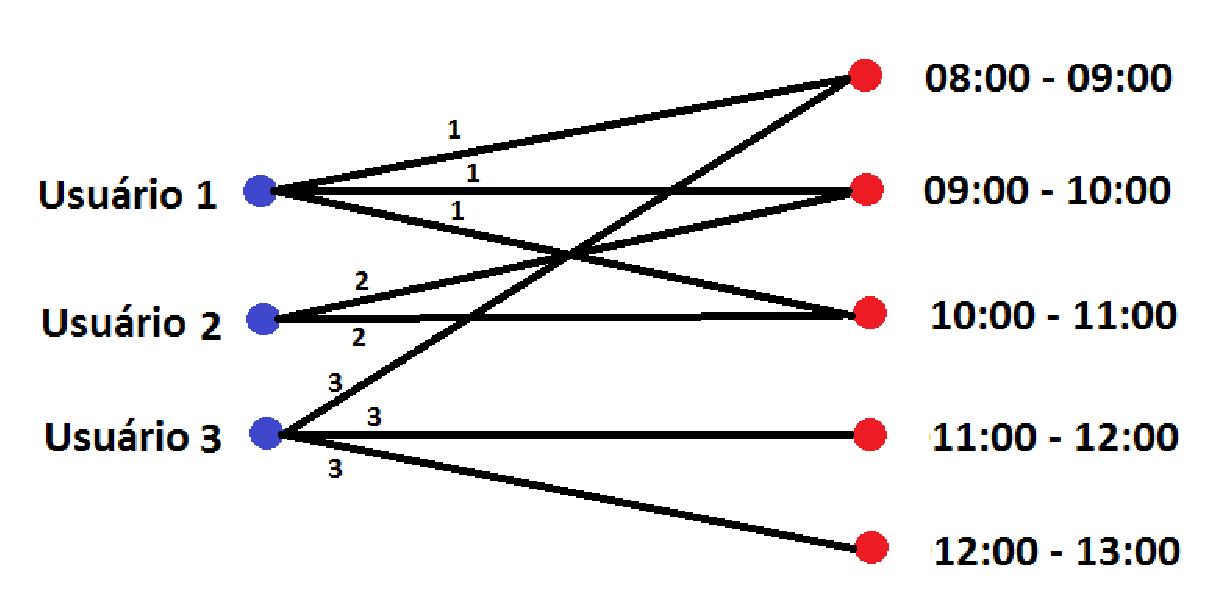
\includegraphics[scale=0.6]{figuras/social_framework/melhor_horario.eps}
    \caption{Exemplo de um grafo bipartido para o problema de melhor horário}
    \label{melhor_horario}
\end{figure}

O peso máximo assumido para os usuários é definido na variável `max\_weight\_schedule' no \textit{initializer} `social\_framework.rb'. Existe também o valor `:fixed' para peso dos usuários. Esse valor representa que é obrigatório que o usuário esteja presente no evento que se deseja marcar.

A verificação do melhor horário para a marcação de eventos foi implementada através do método `verify\_availabilities' da classe `ScheduleContext', com a seguinte assinatura:

\begin{lstlisting}[
    label=listing:change_participant_role,
    caption=Método para mudar o papel de um usuário,
    numbers=none,
    language=Ruby,
    basicstyle=\footnotesize\sffamily,
    keywordstyle=\color{red},
    stringstyle=\color{blue},
    showspaces=false,
    showstringspaces=false,
]
verify_availabilities(users, start_day, finish_day, start_hour = Time.parse("00:00"), finish_hour = Time.parse("23:59"), slots_size = SocialFramework.slots_size)
\end{lstlisting}

O parâmetro `users' representa os usuários que terão suas agendas verificadas, no intuito de encontrar o melhor horário para uma possível marcação de evento. Este parâmetro pode ser um \textit{array}, onde nenhum usuário possui peso no evento ou pode ser uma \textit{hash}, onde a chave é o usuário e o valor é o peso de sua presença no evento.

O parâmetro `start\_day' indica a partir de qual dia o evento poderá ser marcado, e o parâmetro `finish\_day' indica o dia limite para a marcação do evento. O parâmetro `start\_hour' e o parâmetro `finish\_hour' definem o horário de um dia em que o evento poderá ocorrer. Por exemplo pode-se definir o horário comercial de 08:00 às 18:00. Caso estes valores não sejam passados como parâmetros, será considerado que o evento poderá ser marcado em qualquer horário.

O parâmetro `slots\_size' indica o tempo de duração dos \textit{slots}. Caso não seja passado como parâmetro, é utilizado o tempo padrão, definido no arquivo configuração e com duração de 1 hora.

A quantidade de \textit{slots} que serão adicionados no grafo depende do intervalo de tempo em que se deseja analisar e do tempo de duração de cada \textit{slot}.

Para criar as arestas entre os usuários e os \textit{slots}, é verificado se o usuário possui disponibilidade em sua agenda no intervalo de tempo que o \textit{slot} possui. Caso o usuário possua disponibilidade para esse \textit{slot}, é criada uma aresta entre o usuário e o \textit{slot}, e o peso do usuário é adicionado ao peso do \textit{slot}. O método retorna os \textit{slots} ordenados decrescentemente pelo peso.

\subsection{Módulo de Rotas}

Este módulo fornece a lógica para trabalhar com rotas. É utilizada a API do Google Maps\footnote{\url{https://developers.google.com/maps/?hl=pt-br}} para fornecer alguns recursos para este módulo, como construir uma rota e obter uma localização a partir de uma latitude e uma longitude.

Para um usuário criar uma rota, deve-se utilizar o método `create\_route', presente na classe de usuário. A seguir, pode-se visualizar a sua assinatura:

\begin{lstlisting}[
    label=listing:create_route,
    caption=Método para criar uma rota,
    numbers=none,
    language=Ruby,
    basicstyle=\footnotesize\sffamily,
    keywordstyle=\color{red},
    stringstyle=\color{blue},
    showspaces=false,
    showstringspaces=false,
]
create_route(title, distance, locations, mode_of_travel = "driving", accepted_deviation = 0)
\end{lstlisting}


Os parâmetros são o título da rota, a distância que a rota possui e as localizações, sendo esse último parâmetro um \textit{array} de \textit{hashs} com todos os pontos de latitude e longitude para construir rota, a seguir é ilustrado um exemplo do parâmetro \textit{locations}:

\begin{lstlisting}[
    label=listing:locations,
    caption=Exemplo de localizações,
    numbers=none,
    language=Ruby,
    basicstyle=\footnotesize\sffamily,
    keywordstyle=\color{red},
    stringstyle=\color{blue},
    showspaces=false,
    showstringspaces=false,
]
locations = [{latitude: -15.792740000000, longitude: -47.876360000000},
             {latitude: -15.792520000000, longitude: -47.876900000000}]
\end{lstlisting}

O parâmetro `mode\_of\_travel'  representa qual o meio de transporte que será utilizado para percorrer a rota, podendo ser `driving', `bycicling', `walking' ou `transit', o valor padrão é `walking' para viajar de carro. Além disso, existe também o parâmetro `accepted\_deviation' com valor padrão igual a zero. Esse parâmetro diz respeito a quanto uma rota pode ter a sua distância alterada, é usado na comparação de rotas.

Este módulo também fornece um recurso para verificar a compatibilidade entre duas rotas. Para isso, deve-se chamar o método `compare\_routes' presente na classe `RouteContext'.

\begin{lstlisting}[
    label=listing:compare_routes,
    caption=Método para comparar rotas,
    numbers=none,
    language=Ruby,
    basicstyle=\footnotesize\sffamily,
    keywordstyle=\color{red},
    stringstyle=\color{blue},
    showspaces=false,
    showstringspaces=false,
]
compare_routes(principal_route, secondary_route)
\end{lstlisting}

Este método é utilizado para verificar se duas rotas podem ser conectadas em apenas uma rota. O parâmetro `principal\_route' representa a rota que será alterada para auxiliar a rota secundária representada pelo parâmetro `secondary\_route', se possível. Quando a rota principal não pode ser alterada, pode-se tentar alterar a rota secundária para atingir o objetivo. O método utiliza os valores de desvio máximo das rotas para poder verificar se as rotas podem ser desviadas para atender os objetivos esperados.

O método \textit{compare\_routes} retorna um mapa com as informações de compatibilidade, como pode ser visualizado a seguir:

\begin{lstlisting}[
    label=listing:compatible,
    caption=Retorno do método que compara as rotas,
    numbers=none,
    language=Ruby,
    basicstyle=\footnotesize\sffamily,
    keywordstyle=\color{red},
    stringstyle=\color{blue},
    showspaces=false,
    showstringspaces=false,
]
{compatible: false, principal_route: {deviation: :none,
          distance: 0}, secondary_route: {deviation: :none, distance: 0}}
\end{lstlisting}

A chave `compatible' é falsa quando as rotas são incompatíveis ou verdadeira quando são compatíveis. O desvio representa onde a rota poderá ser desviada, podendo ser `none', `both', `origin' ou `destiny'. No caso, `distance' é o valor da distância total que a rota possui com o desvio incluso.

As rotas também podem ser relacionadas aos eventos. Para fazer o relacionamento, deve-se invocar o método `add\_route', presente na classe de evento.

\begin{lstlisting}[
    label=listing:compatible,
    caption=Retorno do método para adicionar uma rota em um evento,
    numbers=none,
    language=Ruby,
    basicstyle=\footnotesize\sffamily,
    keywordstyle=\color{red},
    stringstyle=\color{blue},
    showspaces=false,
    showstringspaces=false,
]
add_route(user, route)
\end{lstlisting}

O primeiro parâmetro é o usuário que tentará adicionar a rota no evento, sendo necessário que o usuário tenha a permissão `add\_route' no evento (as permissões para executar as ações nos eventos estão definidas no \textit{initialize} `social\_framework.rb'). O segundo parâmetro é a rota que será adicionada no evento. Quando uma rota é adicionada a um evento, todos os usuários neste evento recebem essa rota.

\section{Hotspots}
\label{sec:hotspots}

O SocialFramework possui três pontos de \textit{Hotspots} principais. Nesses pontos foram implementados três padrões de projeto para auxiliar na estruturação dos elementos do \textit{framework}. Além dos pontos mencionados, o \textit{framework} é extensível, e permite ao usuário mudar qualquer comportamento padrão implementado através de heranças e sobrescrita de métodos.

O primeiro Hotspot definido para o \textit{framework} está presente nas classes de modelo. Como mencionada nas sessões \nameref{configuracao_das_modelos} e \nameref{configuracao_das_migrations}, é mostrada a possibilidade de se estender uma classe de modelo ou mudar uma \textit{migration} adicionando ou removendo novos atributos para a classe. Porém, existe um problema, quando se estende uma classe de modelo para sobrescrever algum método padrão, essas alterações não serão refletidas para todos os pontos do \textit{framework} onde aquele método é usado. Foi utilizado uma adaptação do \nameref{sec:padrao_factory_method} para resolver este problema. Essa adaptação se deu pelo fato de não ser necessário a criação das classes abstratas, pois as classes que serão instanciadas pela fábrica já representam o comportamento padrão do \textit{framework} e para a fábrica instanciá-las só é necessário nome da classe. Com isso, agora é possível, usando-se a classe \textit{ModelFabric}, dizer qual classe de modelo deve ser construída para ser utilizada. Dessa forma, caso um usuário do \textit{framework} estenda uma classe de modelo qualquer, sobrescrevendo um de seus métodos, este poderá simplesmente chamar o método estático \textit{get\_class}, passando o nome de sua nova classe. E essa classe passará a ser usada pelo \textit{framework}. A seguir, é apresentado um modelo de uso desse método para facilitar o entendimento.

\begin{lstlisting}[
    label=listing:get_class,
    caption=Método para construir nova classe de modelo,
    numbers=none,
    language=Ruby,
    basicstyle=\footnotesize\sffamily,
    keywordstyle=\color{red},
    stringstyle=\color{blue},
    showspaces=false,
    showstringspaces=false,
]
ModelFabric.get_class("NovaClasseModelo")
\end{lstlisting}

Existe outro facilitador desenvolvido no \textit{framework} para trabalhar com o padrão mencionado. Os nomes de todas as classes de modelo estão definidos no \textit{initializer} `social\_framework.rb', sendo assim, quando um desenvolvedor cria uma nova classe de modelo que estende de alguma \textit{model} padrão, basta que mude o nome da respectiva classe nesse arquivo e tudo estará funcionando. Dessa forma, a classe \textit{ModelFabric} se torna transparente para um usuário do \textit{framework}, pois está sendo chamada nos métodos internos, e basta fazer a alteração de nome no arquivo `social\_framework.rb', não se esquecendo, que ao se tratar da classe de usuário, que o nome dessa também deve ser alterado no arquivo `routes.rb' para o Devise saber com qual classe de usuário estará trabalhando.

A seguir na figura \ref{padrao_factory_method}, pode ser visto o diagrama das classes construído para aplicação do padrão.

\begin{figure}[h]
    \centering
    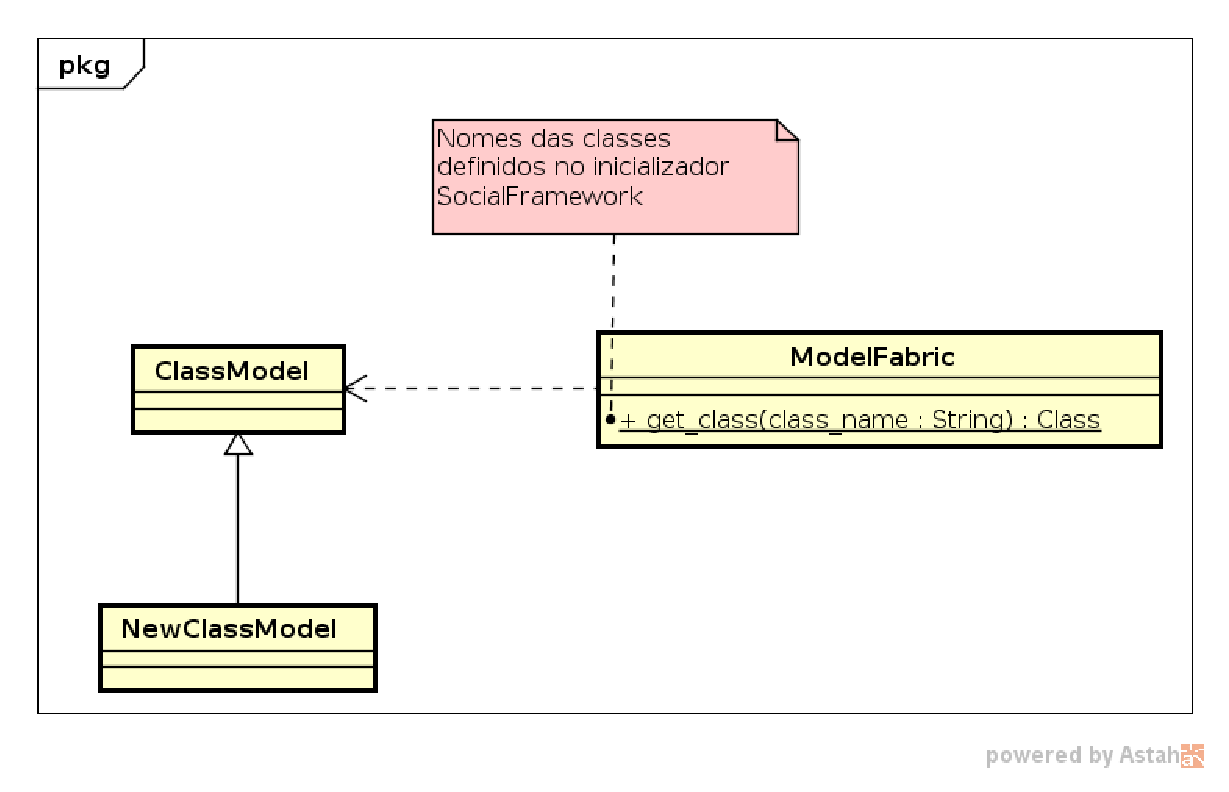
\includegraphics[scale=0.6]{figuras/social_framework/factory_method.eps}
    \caption{Classes no SocialFramework para aplicação do Factory Method}
    \label{padrao_factory_method}
\end{figure}

Outro padrão de projeto de criação utilizado foi o \nameref{sec:padrao_abstract_factory}. Esse padrão foi utilizado para as classes que fazem parte da construção dos grafos, os quais foram utilizados na rede de usuários e na conciliação de agendas para marcação de um horário comum. As classes são \textit{Vertex} e \textit{Edge}. Para cada um delas, existe uma classe abstrata com as assinaturas dos métodos necessários. Também existe a classe abstrata \textit{ElementsFactory} que possui os métodos para criação de \textit{Vertex} e \textit{Edge}.

Para cada classe citada anteriormente, foi desenvolvida uma classe concreta que implementa todos os métodos abstratos com o comportamento padrão esperado para eles. As classes são \textit{VertexDefault}, \textit{EdgeDefault} e \textit{ElementsFactoryDefault} que constrói as duas classes anteriores.

Um desenvolvedor com o intuito de alterar qualquer uma das classes \textit{Vertex} ou \textit{Edge} deve estender essas classes e sobrescrever seus métodos conforme sua necessidade. Deve-se também estender a classe \textit{ElementsFactory} e sobrescrever os métodos de criação, passando suas novas classes. Nas classes que fazem o uso dessas, deve ser passado nas instâncias o novo \textit{ElementsFactory} criado e, assim, as novas classes desenvolvidas passarão a ser utilizadas.

O diagrama com as classes construídas no \textit{framework} para aplicação do padrão \textit{Abstract Factory} pode ser visualizado na Figura \ref{padrao_abstract_factory}.

\newpage
\begin{figure}[h]
    \centering
    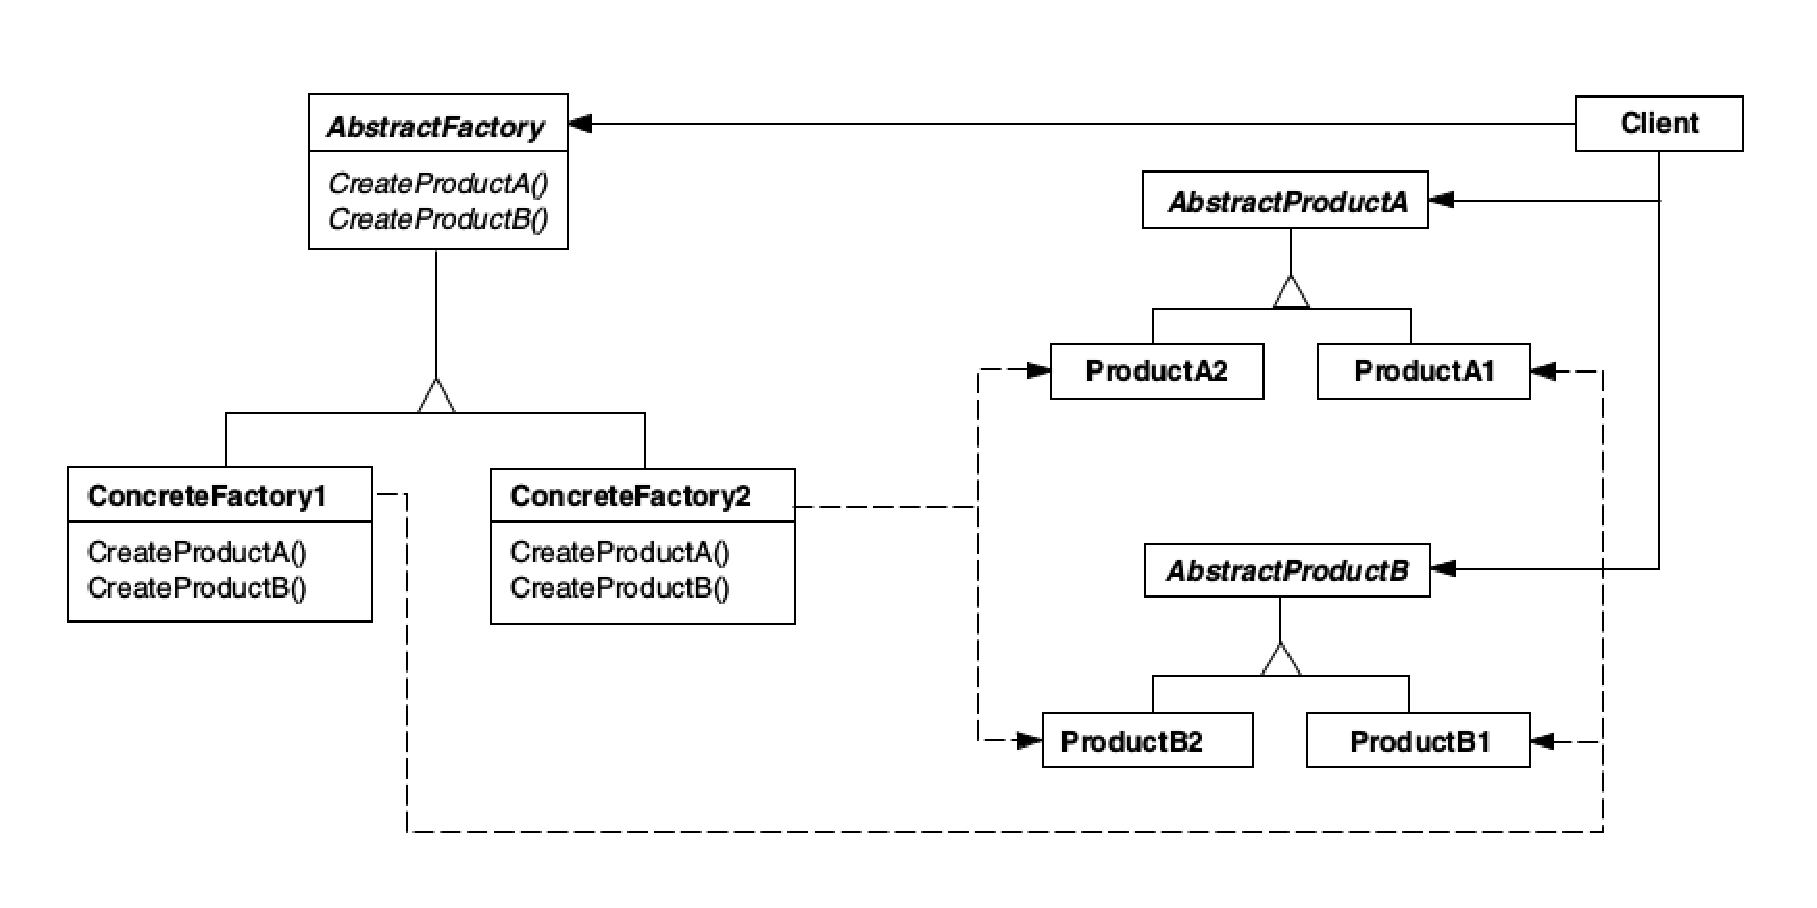
\includegraphics[scale=0.45]{figuras/social_framework/abstract_factory.eps}
    \caption{Classes no SocialFramework para aplicação do Abstract Factory}
    \label{padrao_abstract_factory}
\end{figure}

No diagrama, é mostrado também um exemplo de como seria feita a adição de novas classes que mudem a implementação padrão desenvolvida no \textit{framework}.

Por fim, foi utilizado também o \nameref{sec:padrao_strategy} para cada um dos três módulos do SocialFramework. Para cada um dos módulos, existe uma classe abstrata de estratégia que define todos os métodos públicos do módulo, e uma classe de contexto que será utilizada pelo usuário do \textit{framework}. Essa classe de contexto recebe o tipo de estratégia que será utilizado e o \textit{ElementsFactory} quando for alterado.

Por padrão, o SocialFramework já implementa uma classe de estratégia concreta para cada um dos módulos, e recebe essas classes no construtor de cada classe de contexto. Porém, é simples para que um desenvolvedor altere a estratégia padrão utilizada, basta que esse crie sua nova classe que estenda a classe abstrata de estratégia do módulo e sobrescreva seus métodos, conforme suas necessidades. Adicionalmente, na instanciação da classe de contexto do módulo, deve ser passada a sua nova estratégia, construída através do construtor. Com isso, toda a nova implementação passará a ser usada, sem alteração real alguma sendo feita pelo \textit{framework}.

Os métodos públicos de cada módulo do SocialFramework, que devem ser implementados na mudança de uma estratégia, são descritos detalhadamente nas subseções dos \nameref{sec:modulos_socialframework}. As classes de contexto de cada módulo são: \textit{GraphContext} para o módulo de usuário, \textit{ScheduleContext} para o módulo de agenda, o e \textit{RouteContext} para o módulo de rotas.

A seguir, é apresentada na Figura \ref{padrao_strategy} como está a disposição de classes para os três módulos do SocialFramework.

\begin{figure}[h]
    \centering
    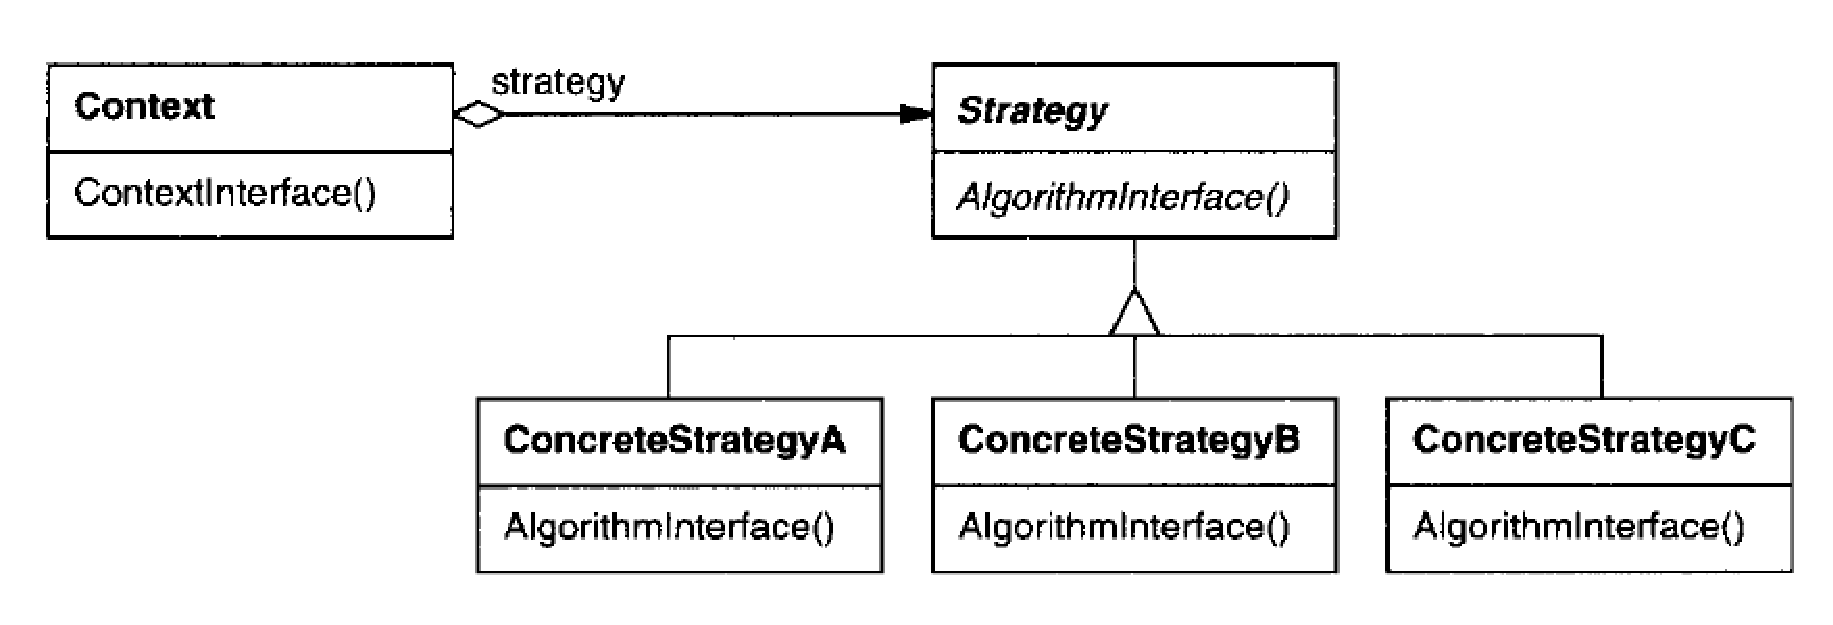
\includegraphics[scale=0.45]{figuras/social_framework/strategy.eps}
    \caption{Classes no SocialFramework para aplicação do Strategy}
    \label{padrao_strategy}
\end{figure}

Em seguida, é apresentado um exemplo de uso quando se altera a estratégia de um módulo.

\begin{lstlisting}[
    label=listing:get_class,
    caption=Instanciação do \textit{ScheduleContext} quando se muda a estratégia,
    numbers=none,
    language=Ruby,
    basicstyle=\footnotesize\sffamily,
    keywordstyle=\color{red},
    stringstyle=\color{blue},
    showspaces=false,
    showstringspaces=false,
]

ScheduleContext.new(NovaEstrategiaDesenvolvida)
\end{lstlisting}

Com isso, ao se chamar o método \textit{verify\_availabilities} dessa classe, estará chamando de fato o método desenvolvido na classe `NovaEstrategiaDesenvolvida'.

Um exemplo de instanciação, com alteração da estratégia e também da fábrica de vértices e arestas, pode ser visualizado abaixo.

\begin{lstlisting}[
    label=listing:get_class,
    caption=Instanciação do \textit{ScheduleContext} quando foram mudadas a estratégia e a fábrica,
    numbers=none,
    language=Ruby,
    basicstyle=\footnotesize\sffamily,
    keywordstyle=\color{red},
    stringstyle=\color{blue},
    showspaces=false,
    showstringspaces=false,
]

ScheduleContext.new(NovaEstrategiaDesenvolvida, NovaFabricaDeElementos)
\end{lstlisting}

Nesse caso, nenhuma das classes padrão do SocialFramework, desenvolvidas para serem usadas no módulo de agenda, estarão sendo usadas, e sim, as novas classes implementadas pelo usuário do \textit{framework}.

\section{Resumo do Capítulo}

Este capítulo apresentou as funcionalidades desenvolvidas para o SocialFramework, passando por toda a sua interface pública e apresentando cada comportamento. Também foi possível conhecer mais a fundo cada módulo que foi proposto e como foram implementados, além dos \textit{Hotspots} criados que trabalham como facilitadores para alterações que se tornem necessárias nas diversas instanciações possíveis do \textit{framework}. A partir dos padrões de projeto implementados nos \textit{Hotspots}, gerou-se uma maior capacidade de reutilização e manutenção do \textit{framework}.
